
\section{Motivation}

The motivation for this thesis mainly includes two parts, in the first part, we illustrate three roots of container-based server consolidation problem. In the second parts, we explain the motivations for solving the sub-problems of the problem.
\begin{itemize}

\item Container is a new virtualization technology which provides an operating level of virtualization.
Figure \ref{fig:root} illustrates the root of container technology from an energy efficient point of view. Most Clouds provide a set fixed types of VM for service providers to choose. Each type of VM represents a certain amount of resources (e.g. CPU, RAM, and Storage). This service model leads to a great waste of resources for two reasons. Firstly, service providers tend to over estimate the resources for ensuring the QoS at the peak hours, hence, they often reserve more resource than they need\cite{Chaisiri:2012wg}. 
Secondly, specific types of application may use a type of resources a lot more than another \cite{Tomas:2013iv}, for example, computation intensive tasks consume CPU much more than RAM; a fixed type of VM may provides much more RAM than it needs. In order to solve this problem, overbooking strategy tends to place more VMs than the server's maximum capacity. However, this technique is highly relied on the workload prediction running in a VM. Otherwise, servers are easily overloaded. Container technique can improve the utilization by further partitioning VM into resource isolated chunks. Therefore, multiple applications can share the same VM. This technique avoids the prediction of workload as well as improving the utilization. However, it also need consolidation technique to ensure the high utilization.

\begin{figure}
	\centering
	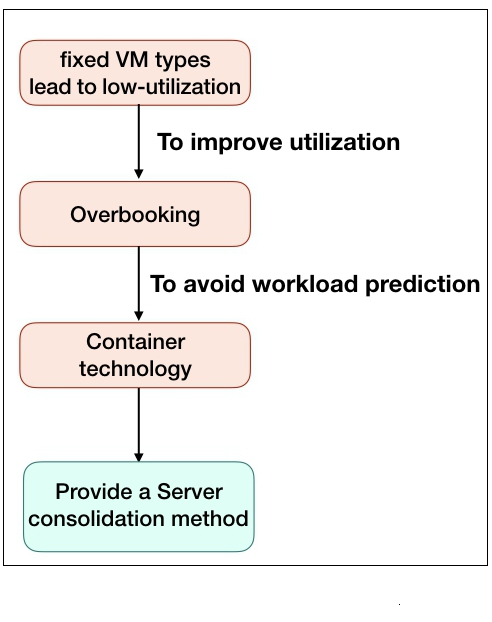
\includegraphics[width=0.3\textwidth]{pics/problem_flow.jpeg}
	\caption{The root of container technology}
	\label{fig:root}
\end{figure}

\item This container-based Cloud certainly brings many advantages to current Cloud \cite{Felter:2015wl}. However, it also brings difficulties for server consolidation. Server consolidation problems are typically modeled as vector bin-packing problem which are NP-hard. Container-based server consolidation add another level of abstraction which makes it a two-level vector bin-packing problem. Current server consolidation methods are mostly VM-based which can not be directly applied on this problem, because two-level of bin-packing problems are interact with each other. Piraghaj \cite{Piraghaj:2016tl} proposes a two-step procedure, mapping tasks to VMs and allocation of VMs. As Mann illustrated in \cite{Mann:2016hx},  these two steps should be conducted simultaneously, otherwise it leads to local optimal. Other research \cite{} propose greedy-based heuristics on this problem. They are relatively fast in execution, but they can be easily stuck at local optimal. 

\end{itemize}

Traditional Cloud computing offers three services models: Infrastructure as a Service (IaaS), Platform as a Service (PaaS) and Software as a Service (SaaS). Both IaaS and PaaS describe how does a service provider use the cloud resources. The main difference of these two models are  
IaaS allows service providers to manage the low-level details including the operating system and libraries. While, PaaS provides a higher level of abstraction where users only focus on the application development without caring the underlying operating system and system-level of resources such as CPU cores and memories. However, one drawback of PaaS is that cloud users must make sure their applications are complete compatible with the platform. And in many of the cases, it is not the situation. In order to solve this problem, a container-based virtualization technology starts to reform the Cloud industry. Container as a Service (CaaS) 
is a new concept but it has been used in industry for many years. Containers provide an operating system-level of isolation environment for applications. It does not need a hypervisor but complete rely on the operating system. 


This exciting new technology has bring so many advantages for both Cloud users and Cloud providers. From the providers' perspective, In a large system, running VMs means there are probably many same operating systems occupying memories and storages. Lightweight containers share operating system and therefore, there are more rooms for softwares. It increases the capability of Cloud data centers. Furthermore, in terms of resource utilization, it provides much finer granularity operation than a VM-based Cloud model. Containers partition
a VM into smaller chunks so that with appropriate management, better energy efficiency can be achieved. From the cloud users' perspective, each container provides separated libraries for specific application.  Therefore, it does not contrained by the underlying platform. Like PaaS, Cloud users do not need to concern the scalability of applications. 
Therefore, CaaS can potentially become one of the main stream in the future Cloud computing industry. 

Secondly, energy-efficent computing has been the major concern since the begining of computers. Specifially, Cloud computing has become a popular form. Large-scale data centers have been built around the world. A data center can consume huge amount of energies and it needs to improve its energy-efficiency from multiple perspectives. As we discussed in the Introduction, computing servers are one of the major contribution to the energy consumption. 
And according to observation by \cite{}, the average utilization resource are still very low which causes huge energy wastage. As we mentioned above, the container technolgy provides a better way of managing resources, it has the potential to largly improve the utilization than current VM-based Cloud model because it avoids some of the major drawbacks of VM-based model. 

Thirdly, because the container technology is relatively new, previous research are mostly focus on IaaS model and so that the server consolidation has based on the VM-level. However,   

Frist is this new technology of container that can potentially change the landscape of
Cloud computing. It has so many benefits but also it brings difficulty in managing resources.

Second, from green computing point of view, we still need to manage resource so that, the 
data centers consume less energy. And container technolgy actually bring a better chance to
be more energy-efficient than previous VM based technology.
Third, it is very difficult to manage this container-based resources because of the problem-nature is too complicated. And existed algorithms can not be directly applied on it.
Fourth, the evolutioanry computation provides a good framework to handle such difficult problem.

% \textcolor{Blue}{Motivation is what is now lack from the literature.} \\

% The advantage of Platform as a Service (PaaS) has been discovered in the recent years. 
The disadvantage of tranditional IaaS model has been discovered in the recent years \cite{Mann:2016hx}.
In IaaS, on one hand, cloud customers need to manage the low-level details ranging from application capacity estimation,
resource planning and selection and deployment. 
On the other hand, Cloud providers manage resource provisioning and allocation. 
Although these two tasks are seemingly different, 


The container as a Service (CaaS) cloud model has gain increasing attention in the recent years.
However, the energy efficiency in CaaS cloud environment has not been investigate. 
Particularly, the virtual machine and container joint consolidation is the core problem.
Therefore, in this thesis, we will focus on the end-to-end energy-aware server consolidation on container-based
Cloud. In the meanwhile,  a major research direction of large scale server consolidation is also considered. 
The end-to-end server consolidation refers to the server consolidation techniques used
in the different stages throughout the routine Cloud resource management including  initial VM provisioning and placement, dynamic VM placement, and static VM placement:
